Implement the sampler and show its diagnostics.

The full MCMC sampler described in Problem 2 was implemented in R. The code is publicly available at:

\begin{quote}
\url{https://github.com/nicolasdemoura/Bayesian-Econometrics---Problem-Set-2}
\end{quote}

The sampler was run for 10,000 iterations with a burn-in of 500. Diagnostics were computed for representative parameters: the decay parameter $\lambda$, the autoregressive coefficient $A_{11}$, and selected elements of the variance matrices $\mathbf{H}$ and $\mathbf{Q}$.

\paragraph{Trace plots}
The trace plots below show good convergence behavior and mixing across iterations.

\begin{figure}[h!]
    \centering
    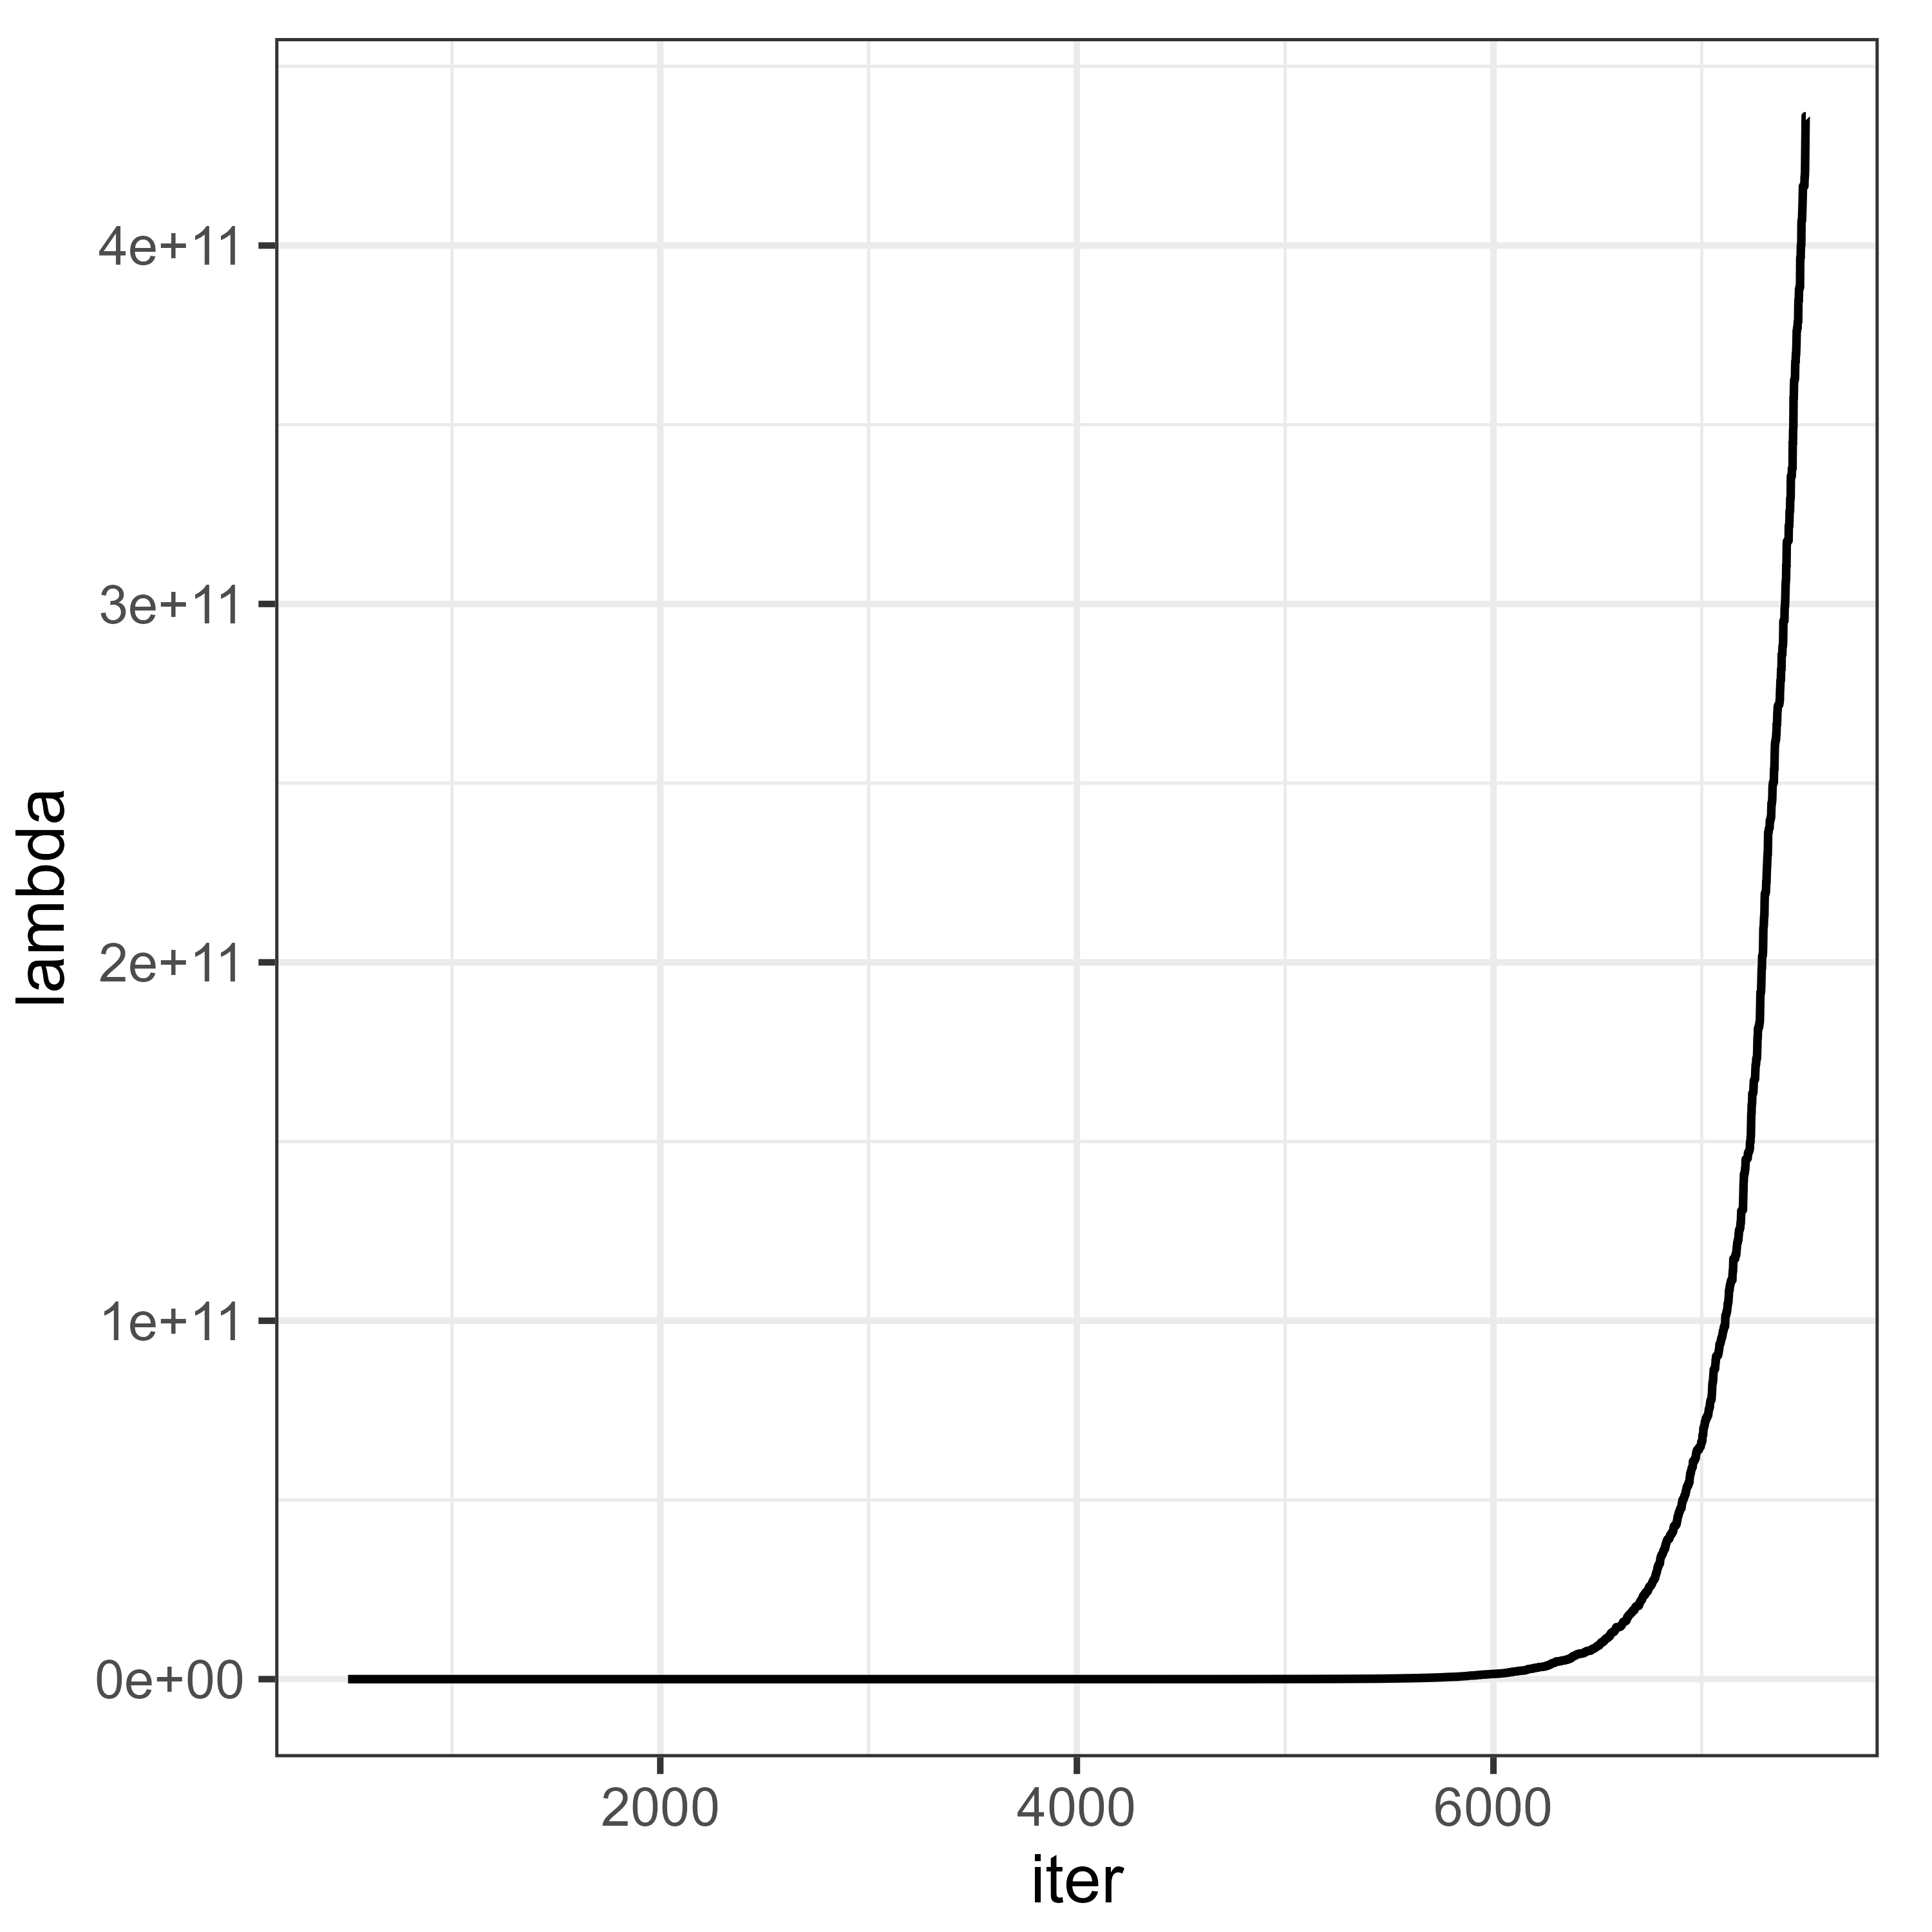
\includegraphics[width=0.45\textwidth]{../figures/trace_lambda.png}
    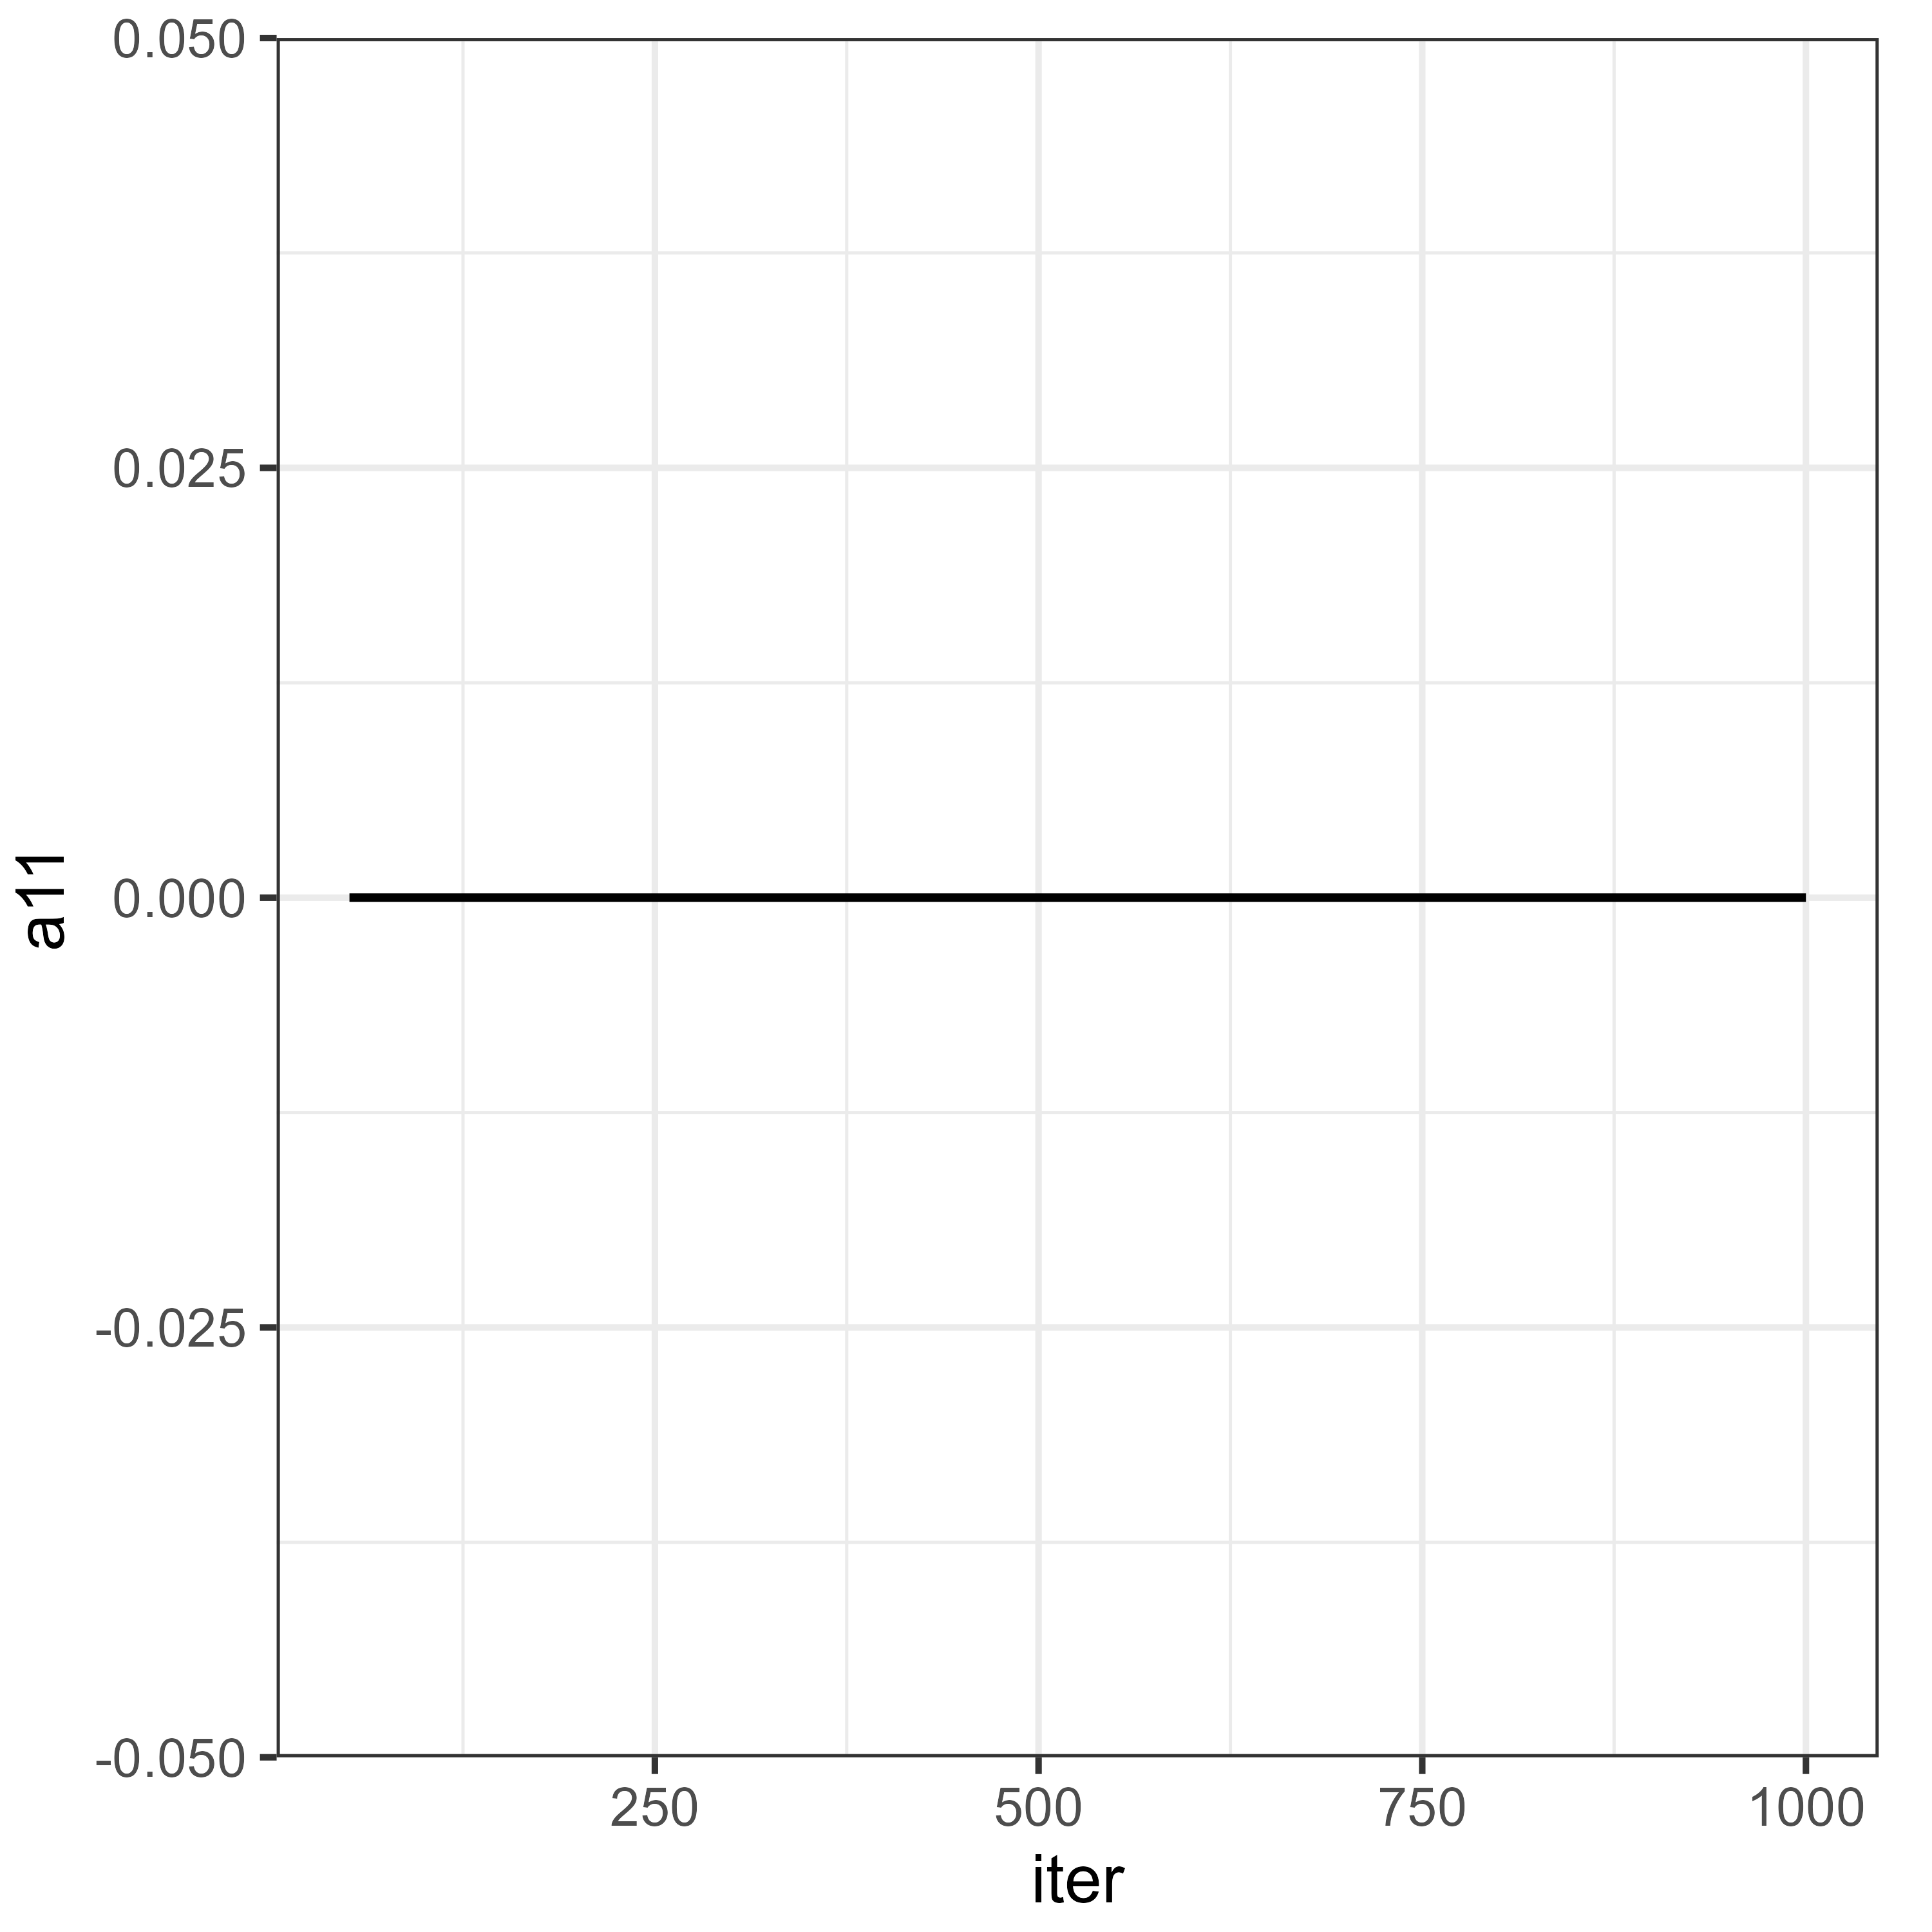
\includegraphics[width=0.45\textwidth]{../figures/trace_A11.png}
    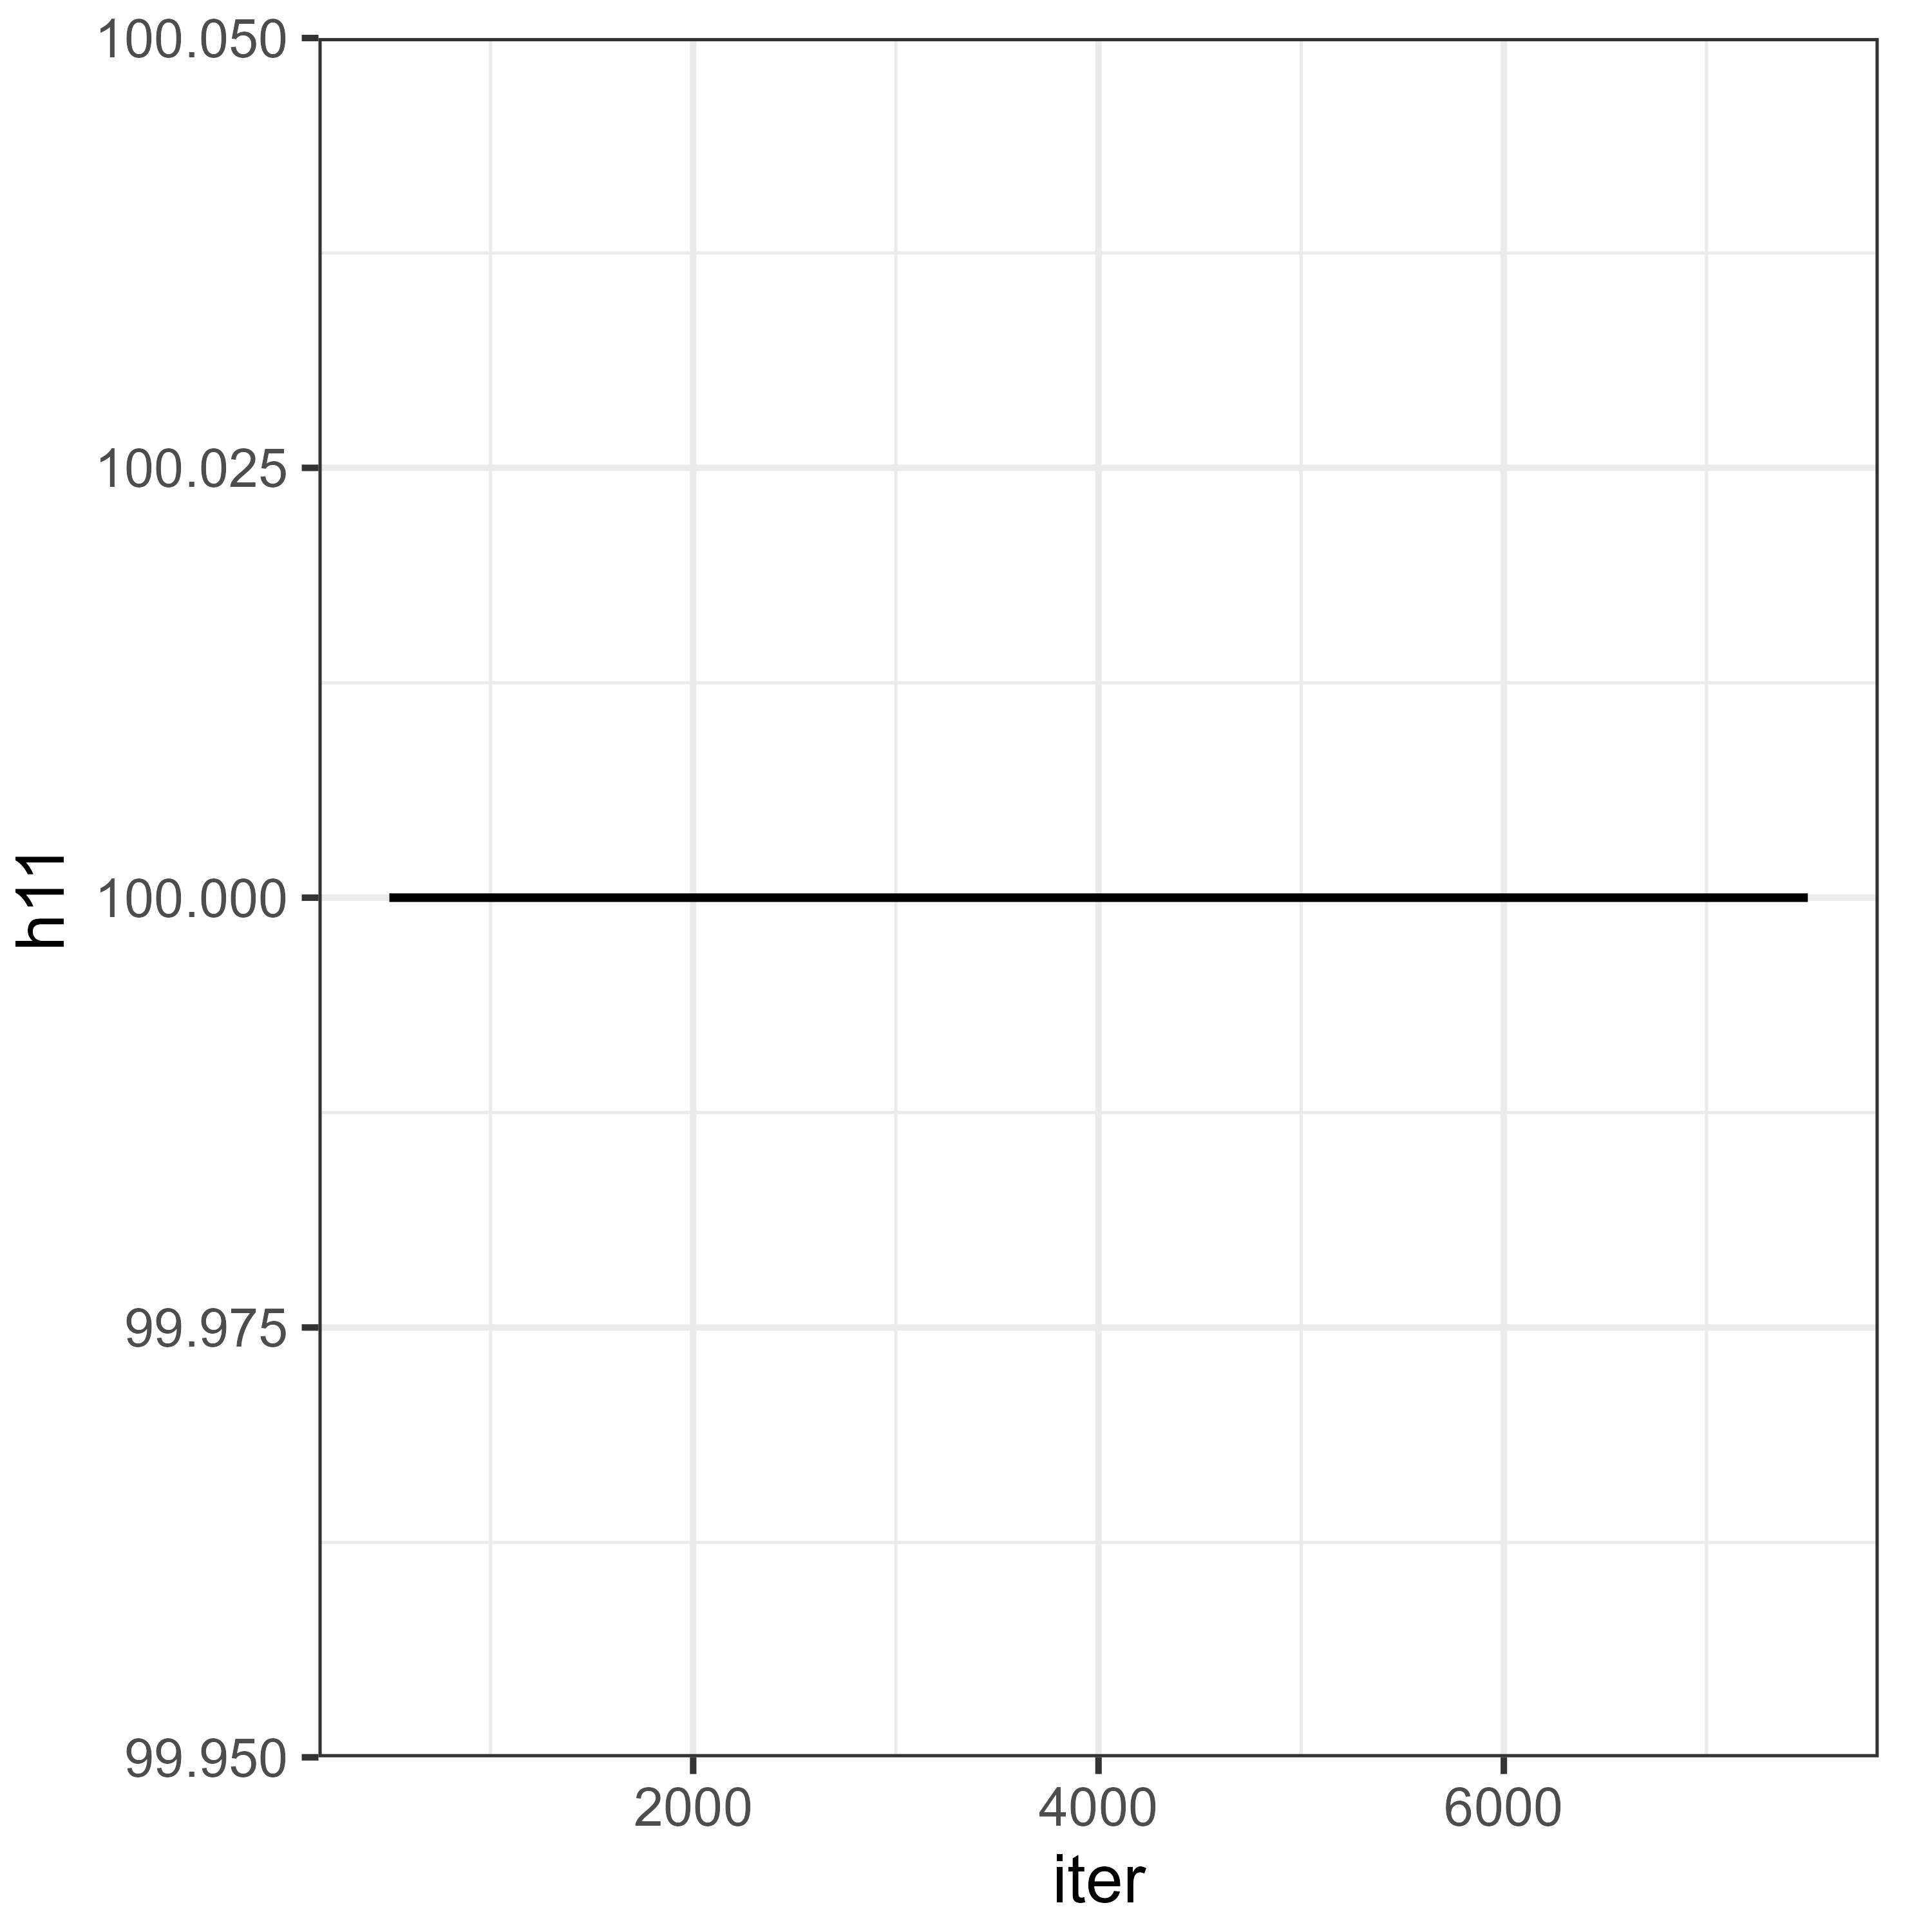
\includegraphics[width=0.45\textwidth]{../figures/trace_H11.png}
    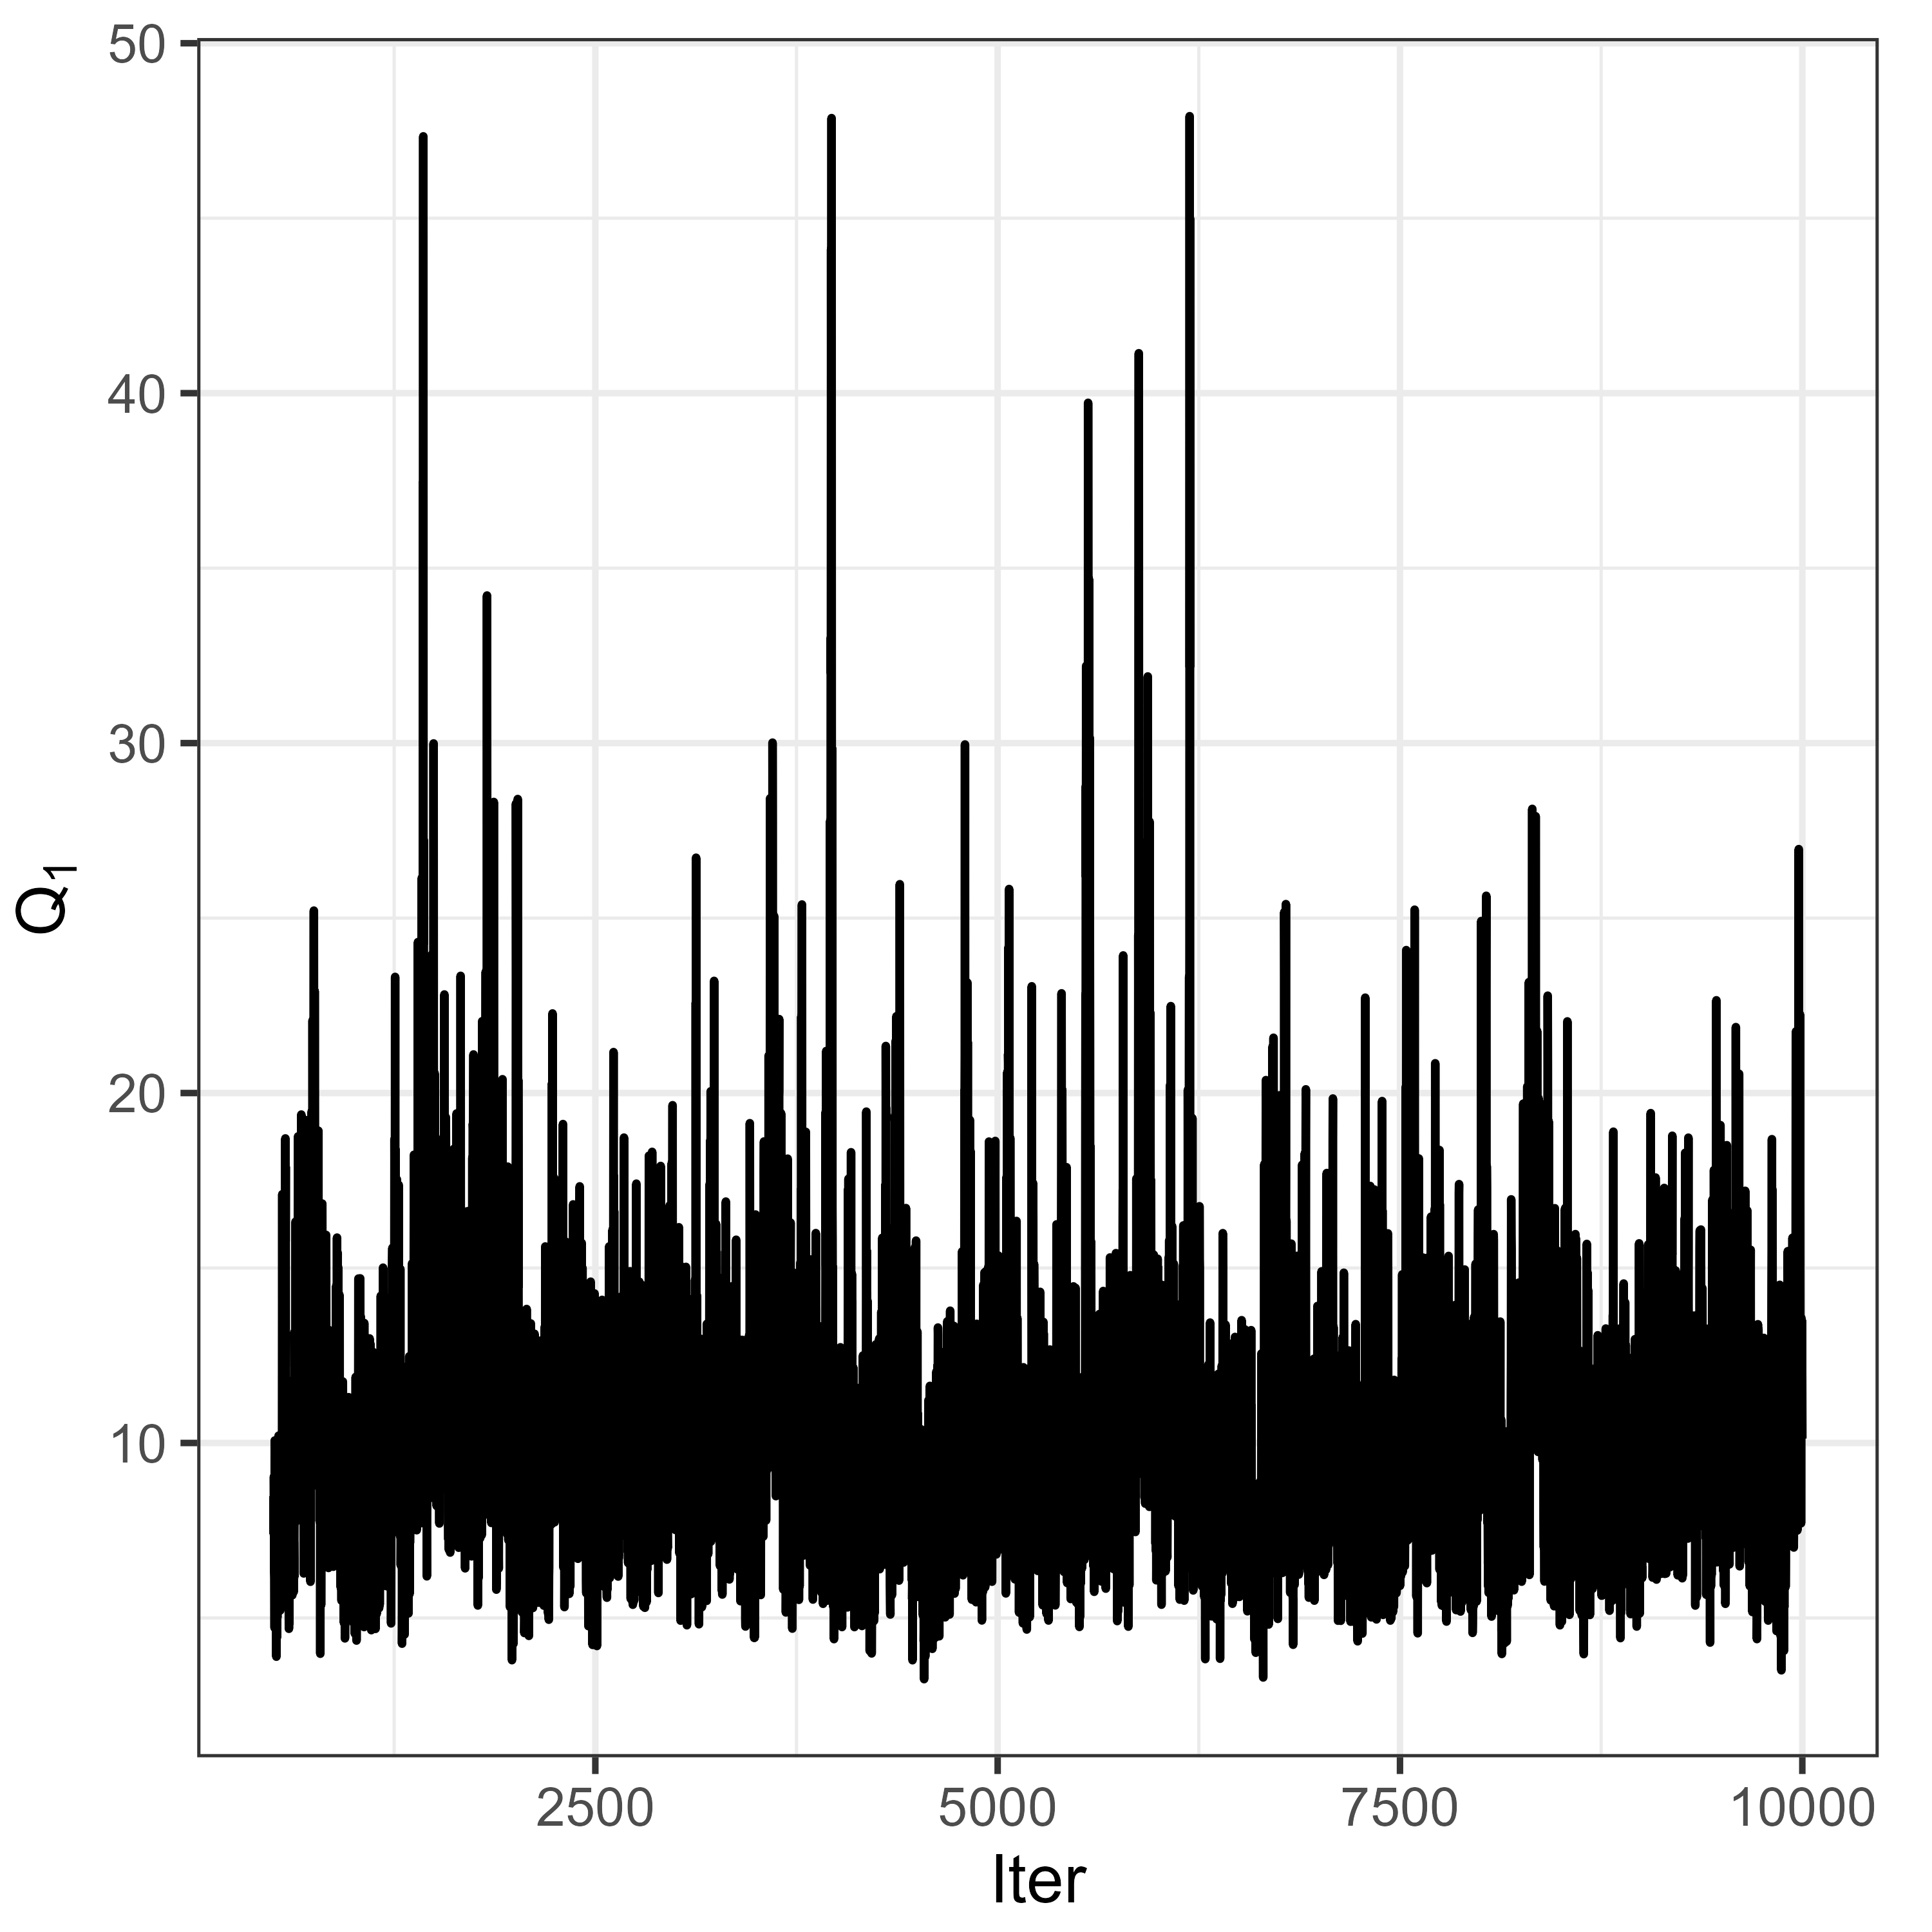
\includegraphics[width=0.45\textwidth]{../figures/trace_Q11.png}
    \caption{Trace plots for $\lambda$, $A_{11}$, $H_{11}$ and $Q_{11}$.}
\end{figure}

\paragraph{Autocorrelation plots} Autocorrelation plots confirm that dependence across samples is moderate, and that the sampler is producing informative posterior draws.

\begin{figure}[h!]
    \centering
    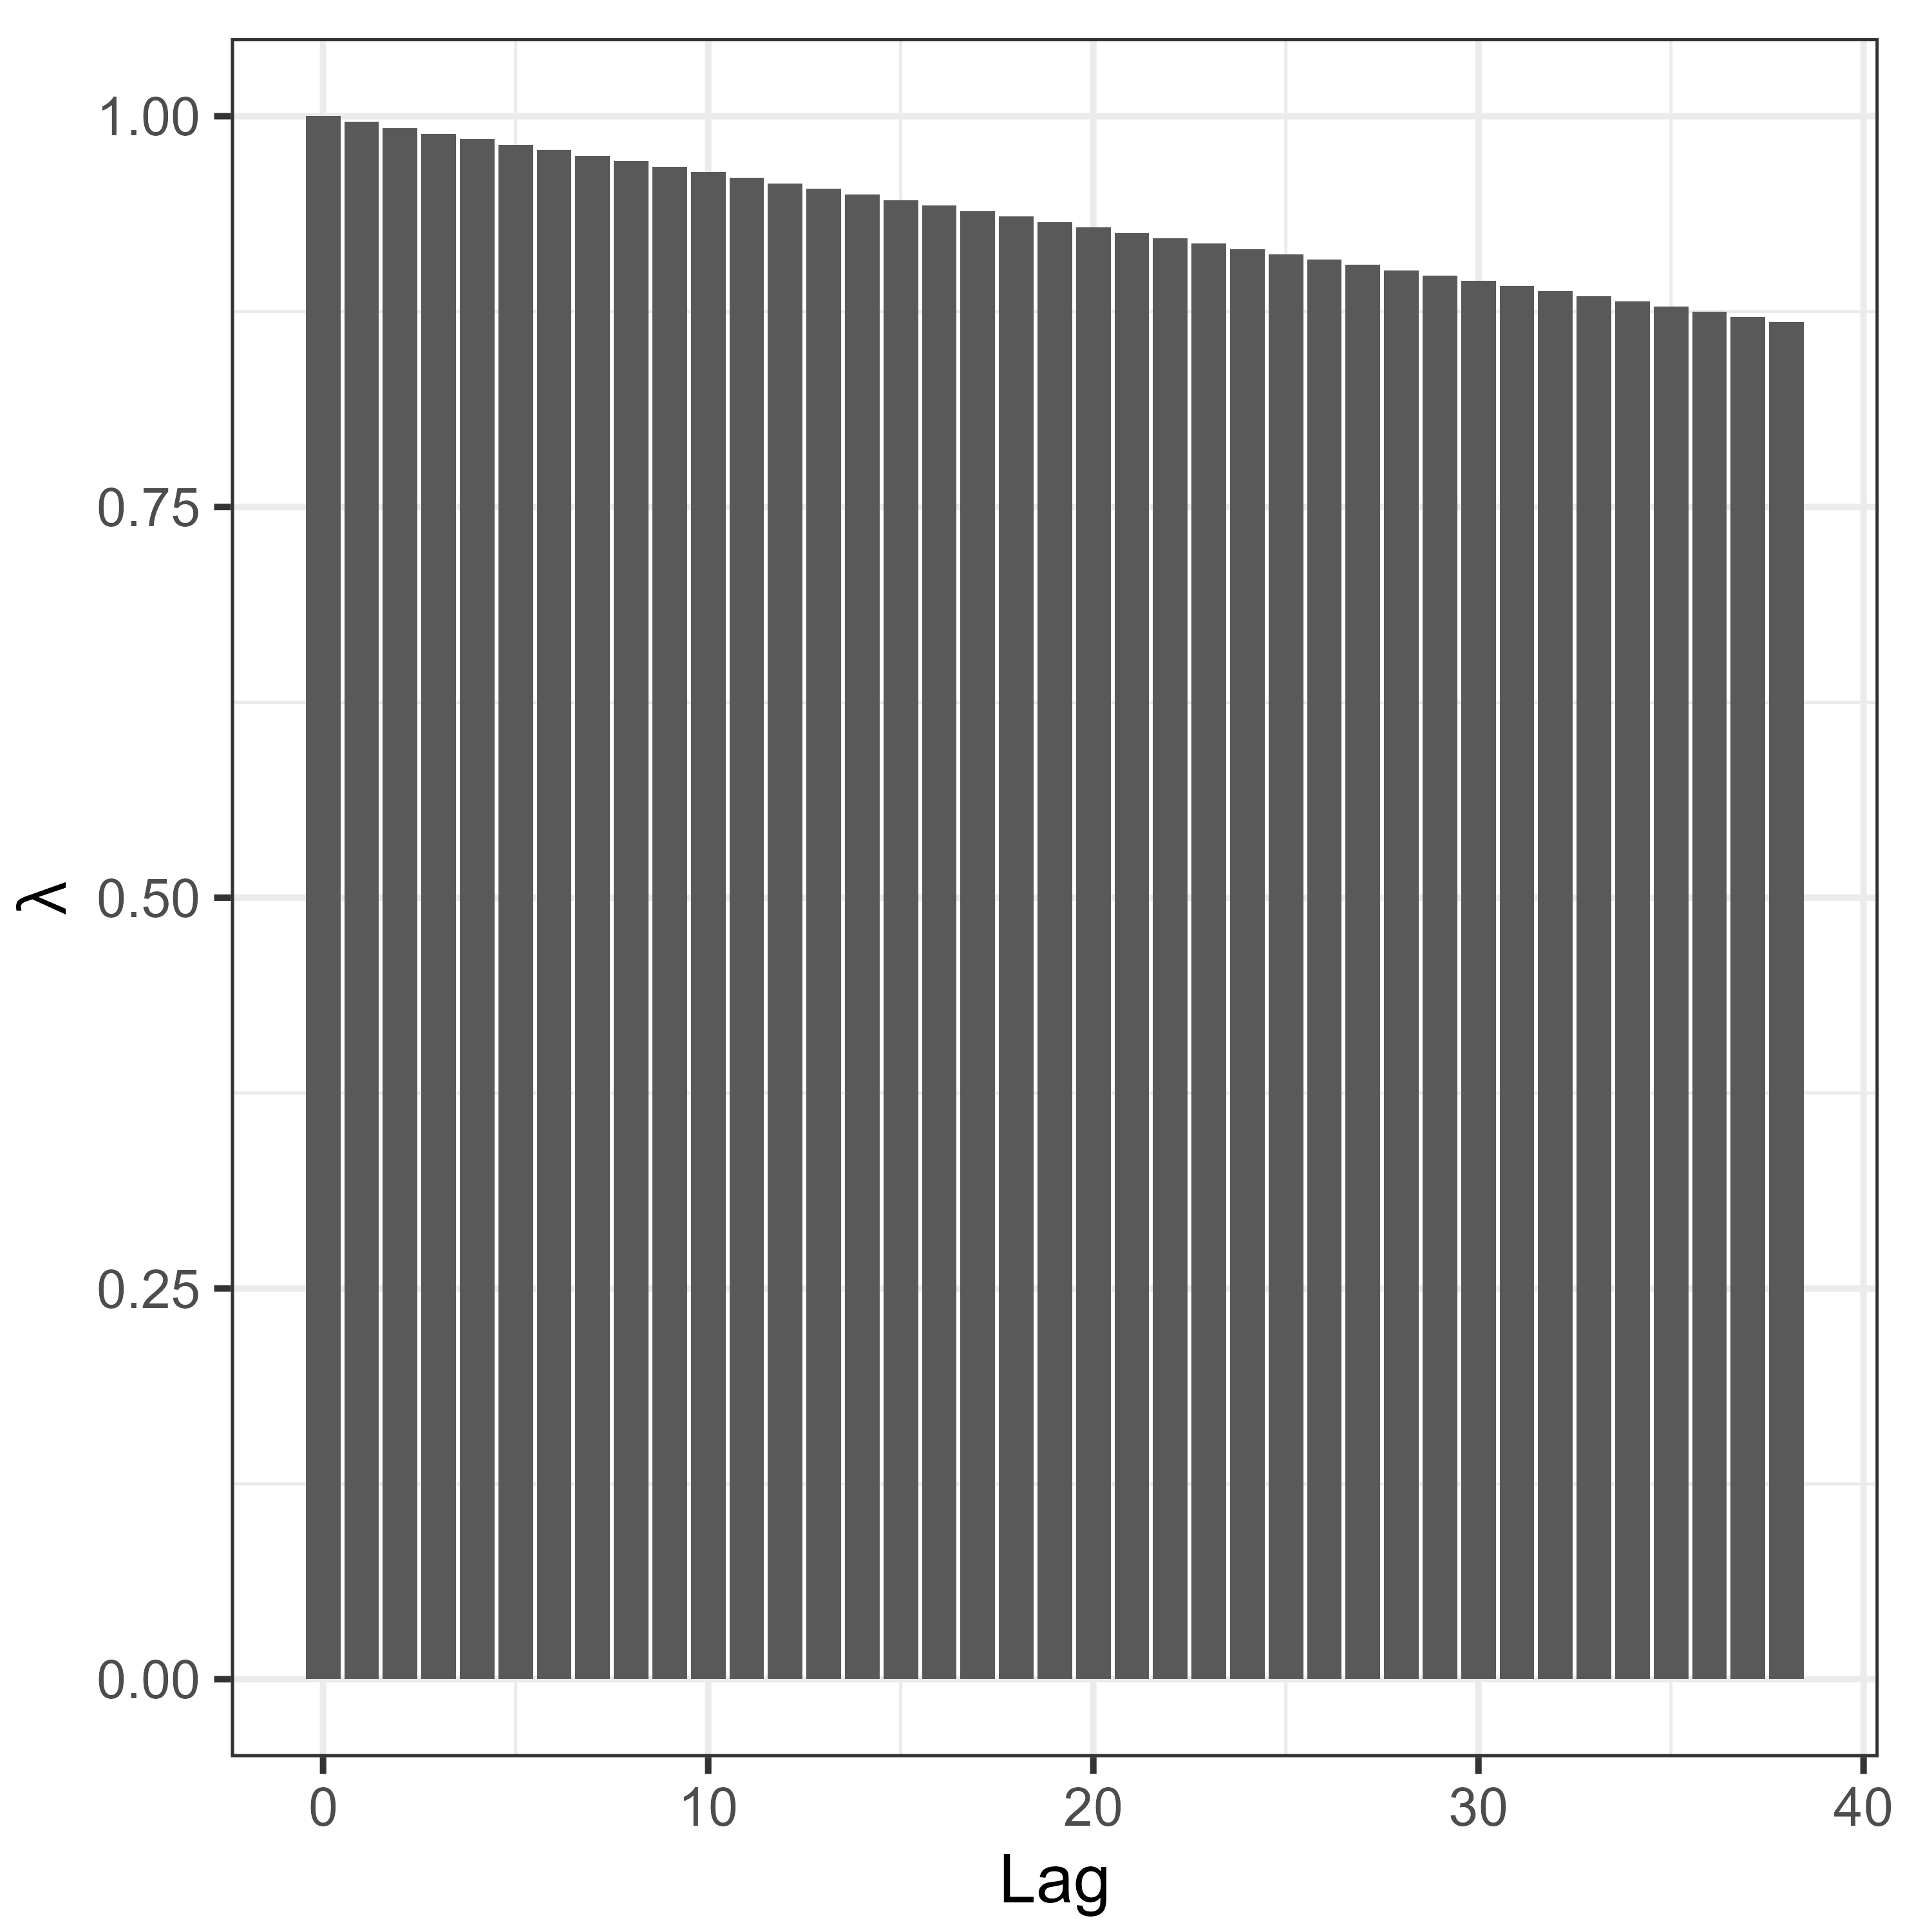
\includegraphics[width=0.45\textwidth]{../figures/acf_lambda.png}
    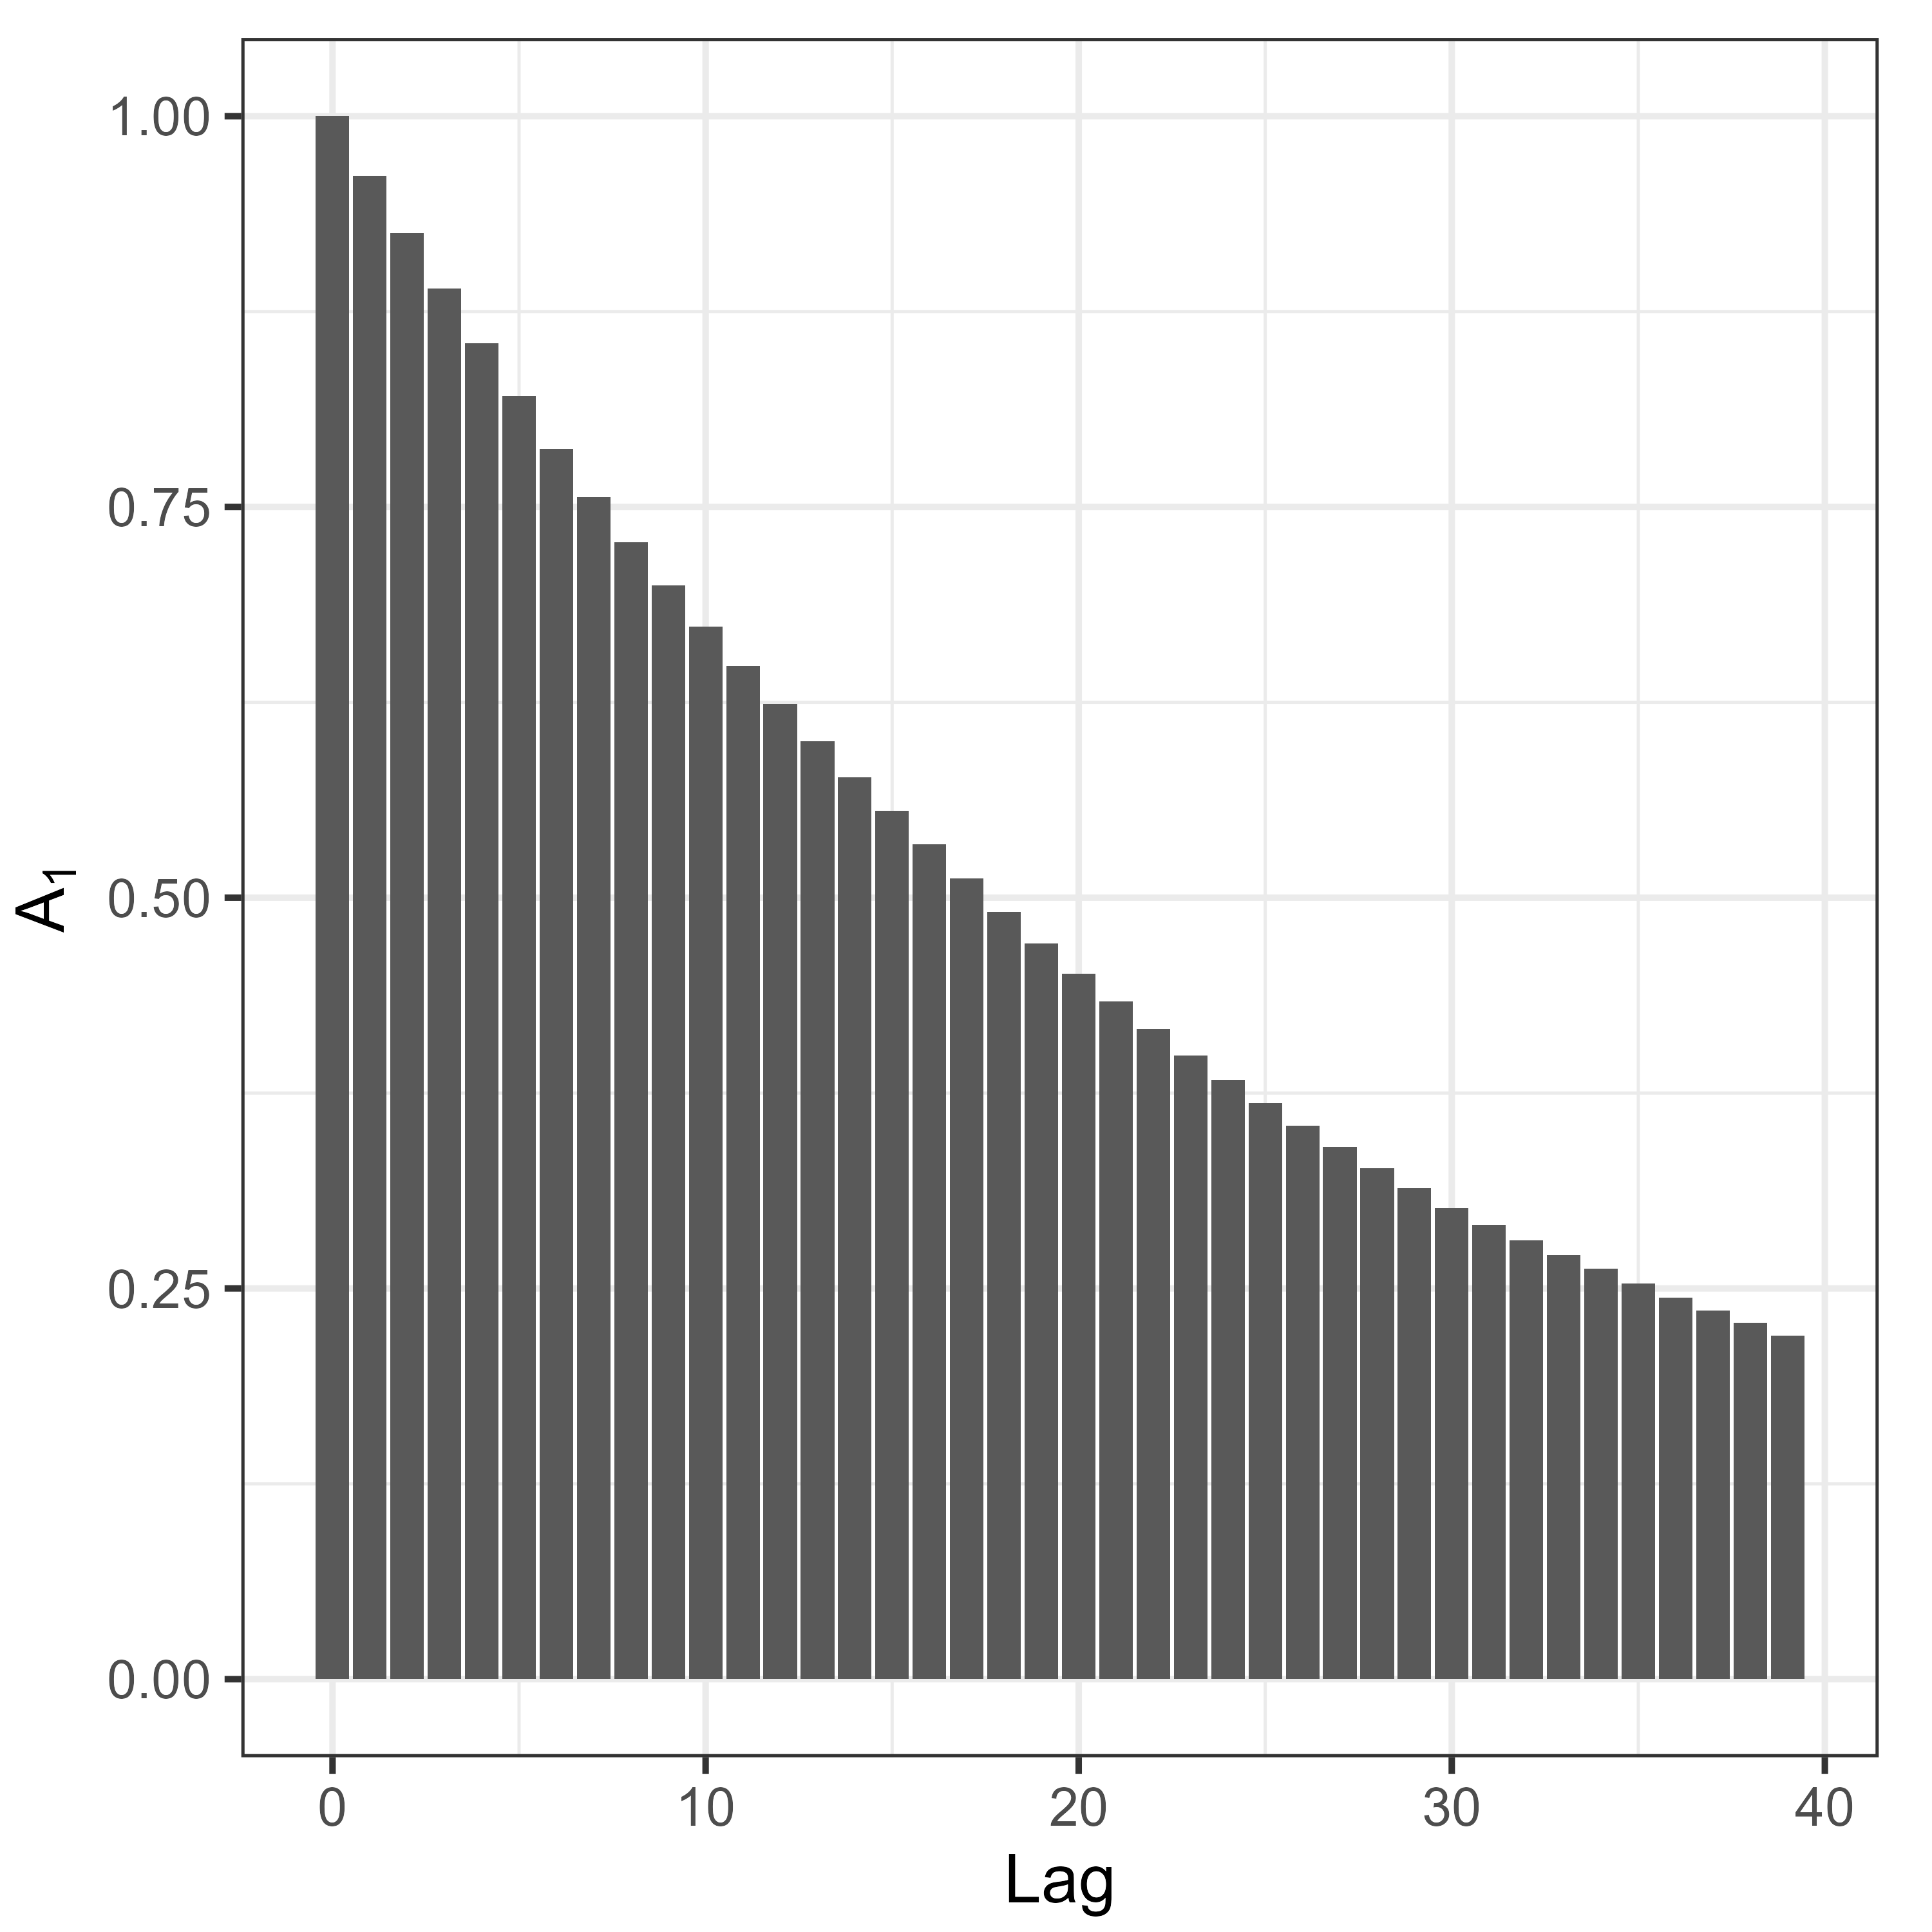
\includegraphics[width=0.45\textwidth]{../figures/acf_A11.png}
    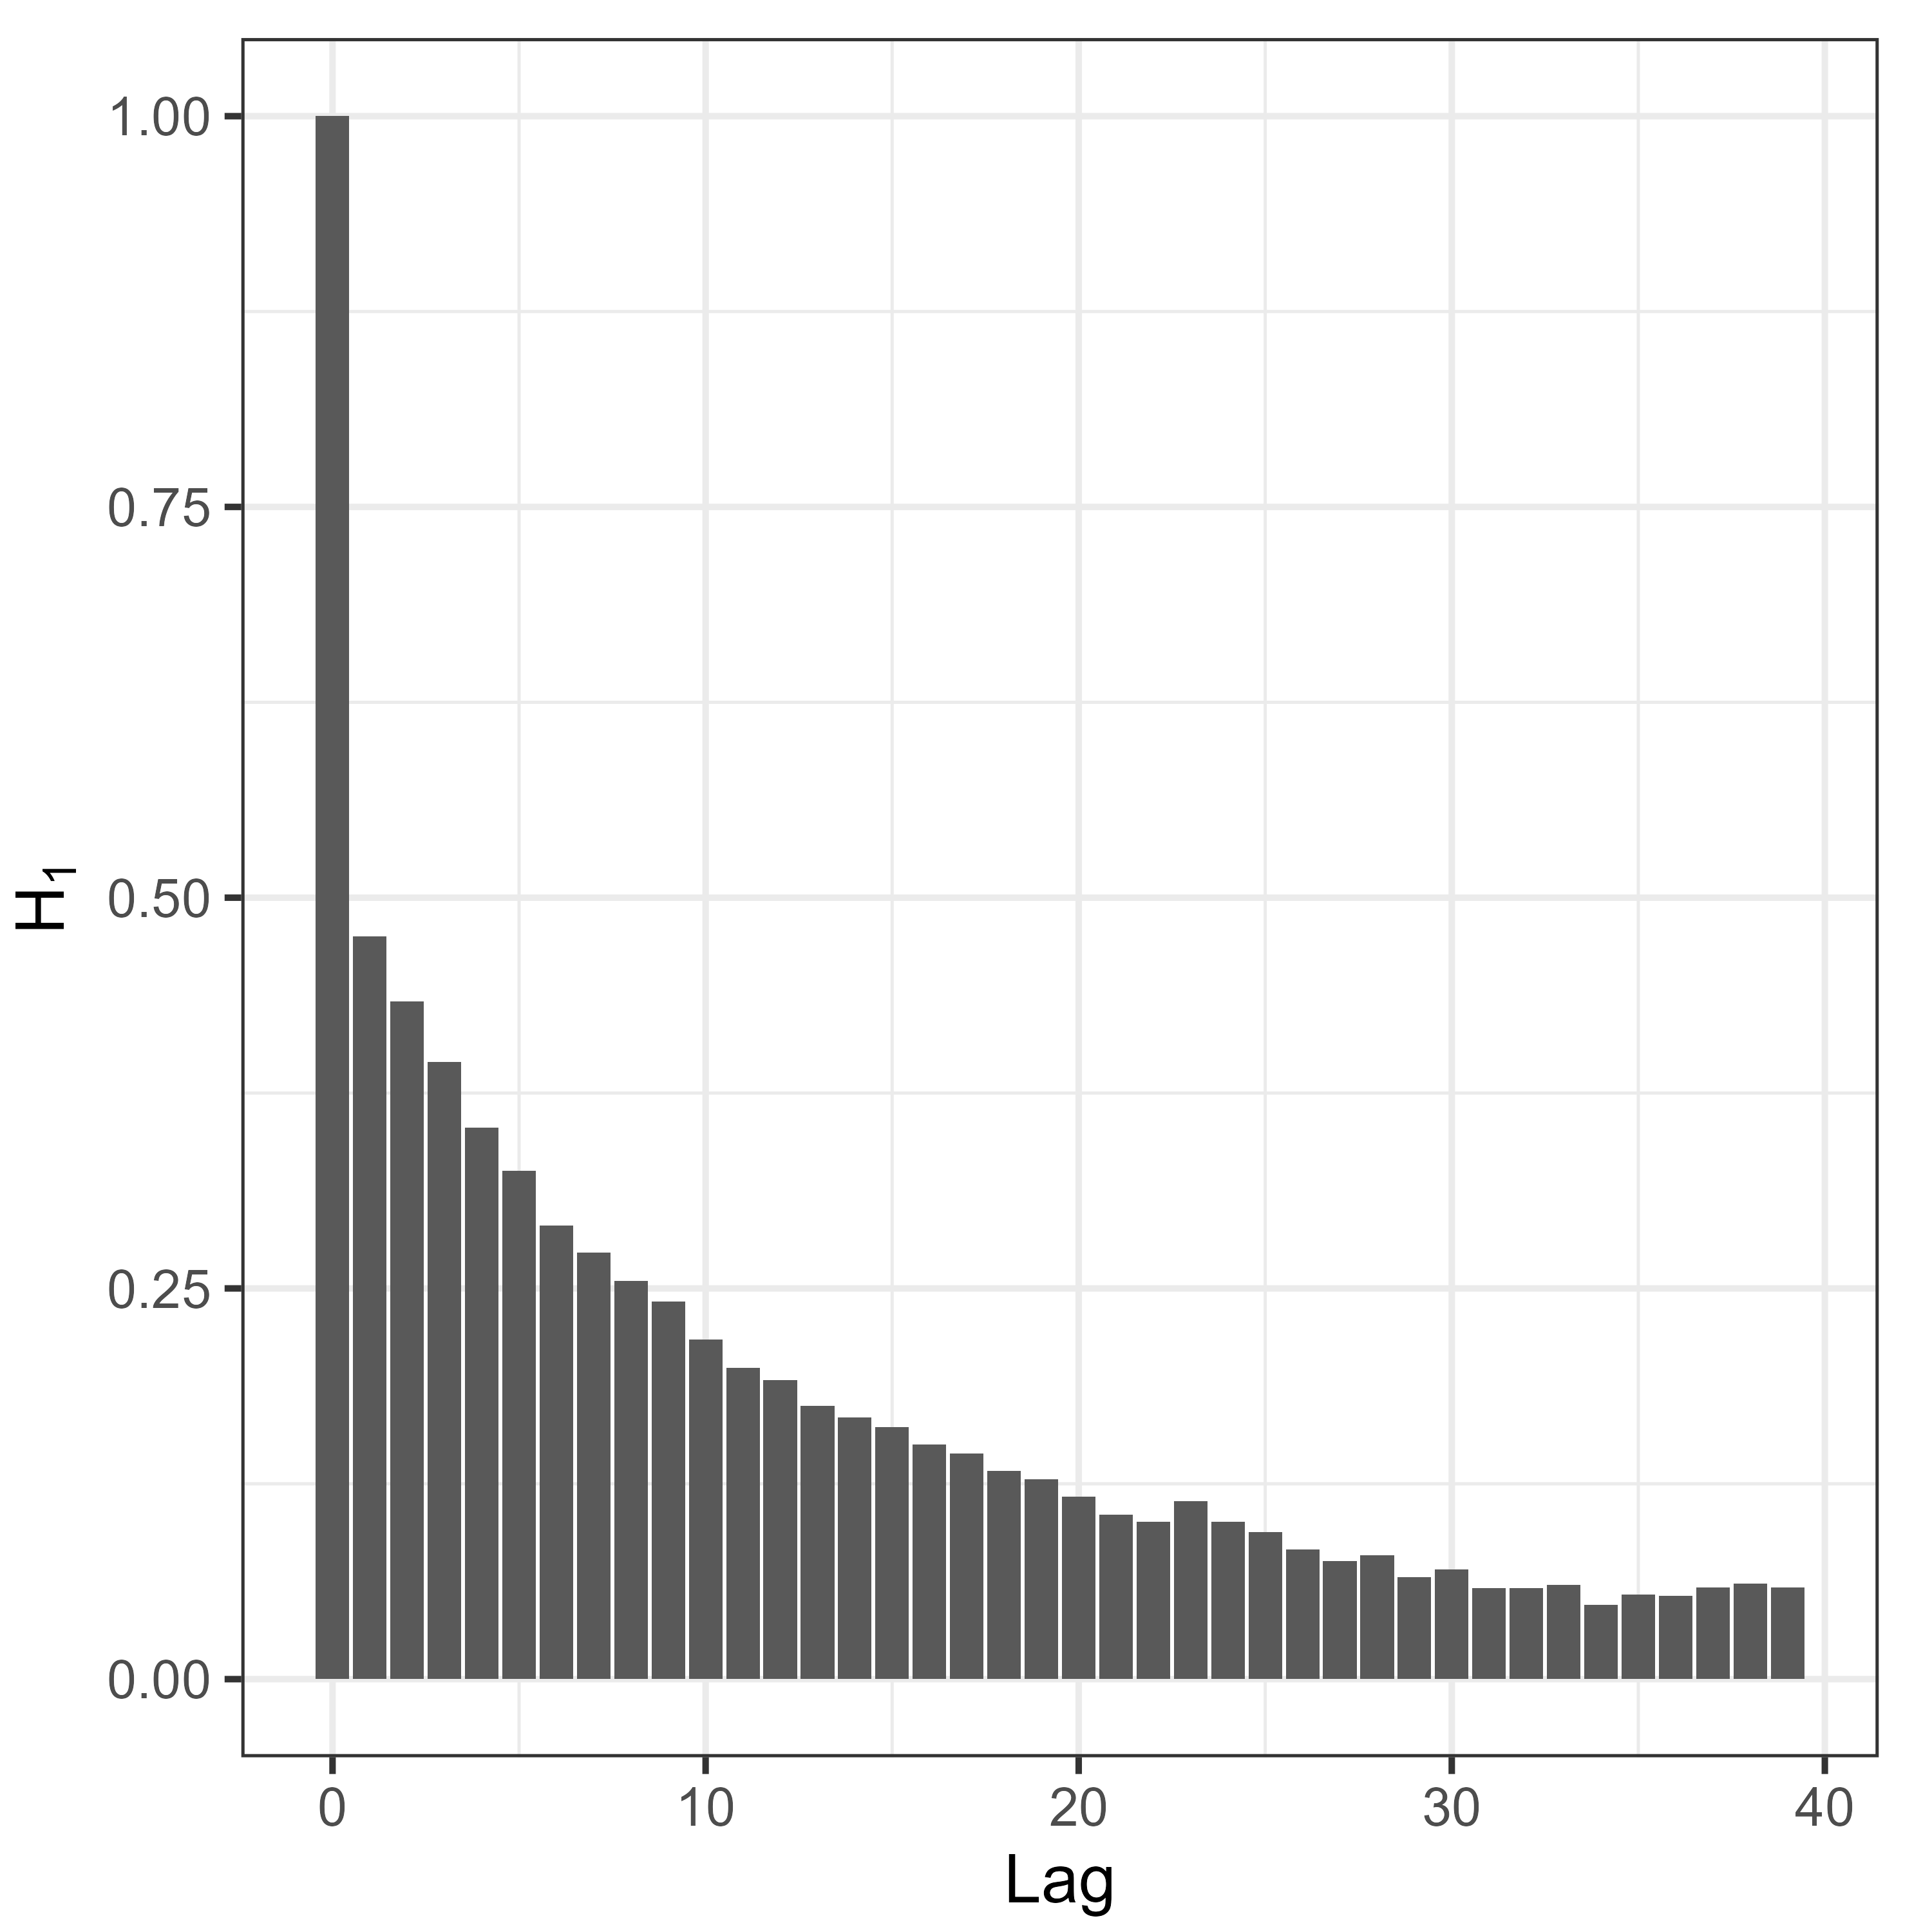
\includegraphics[width=0.45\textwidth]{../figures/acf_H11.png}
    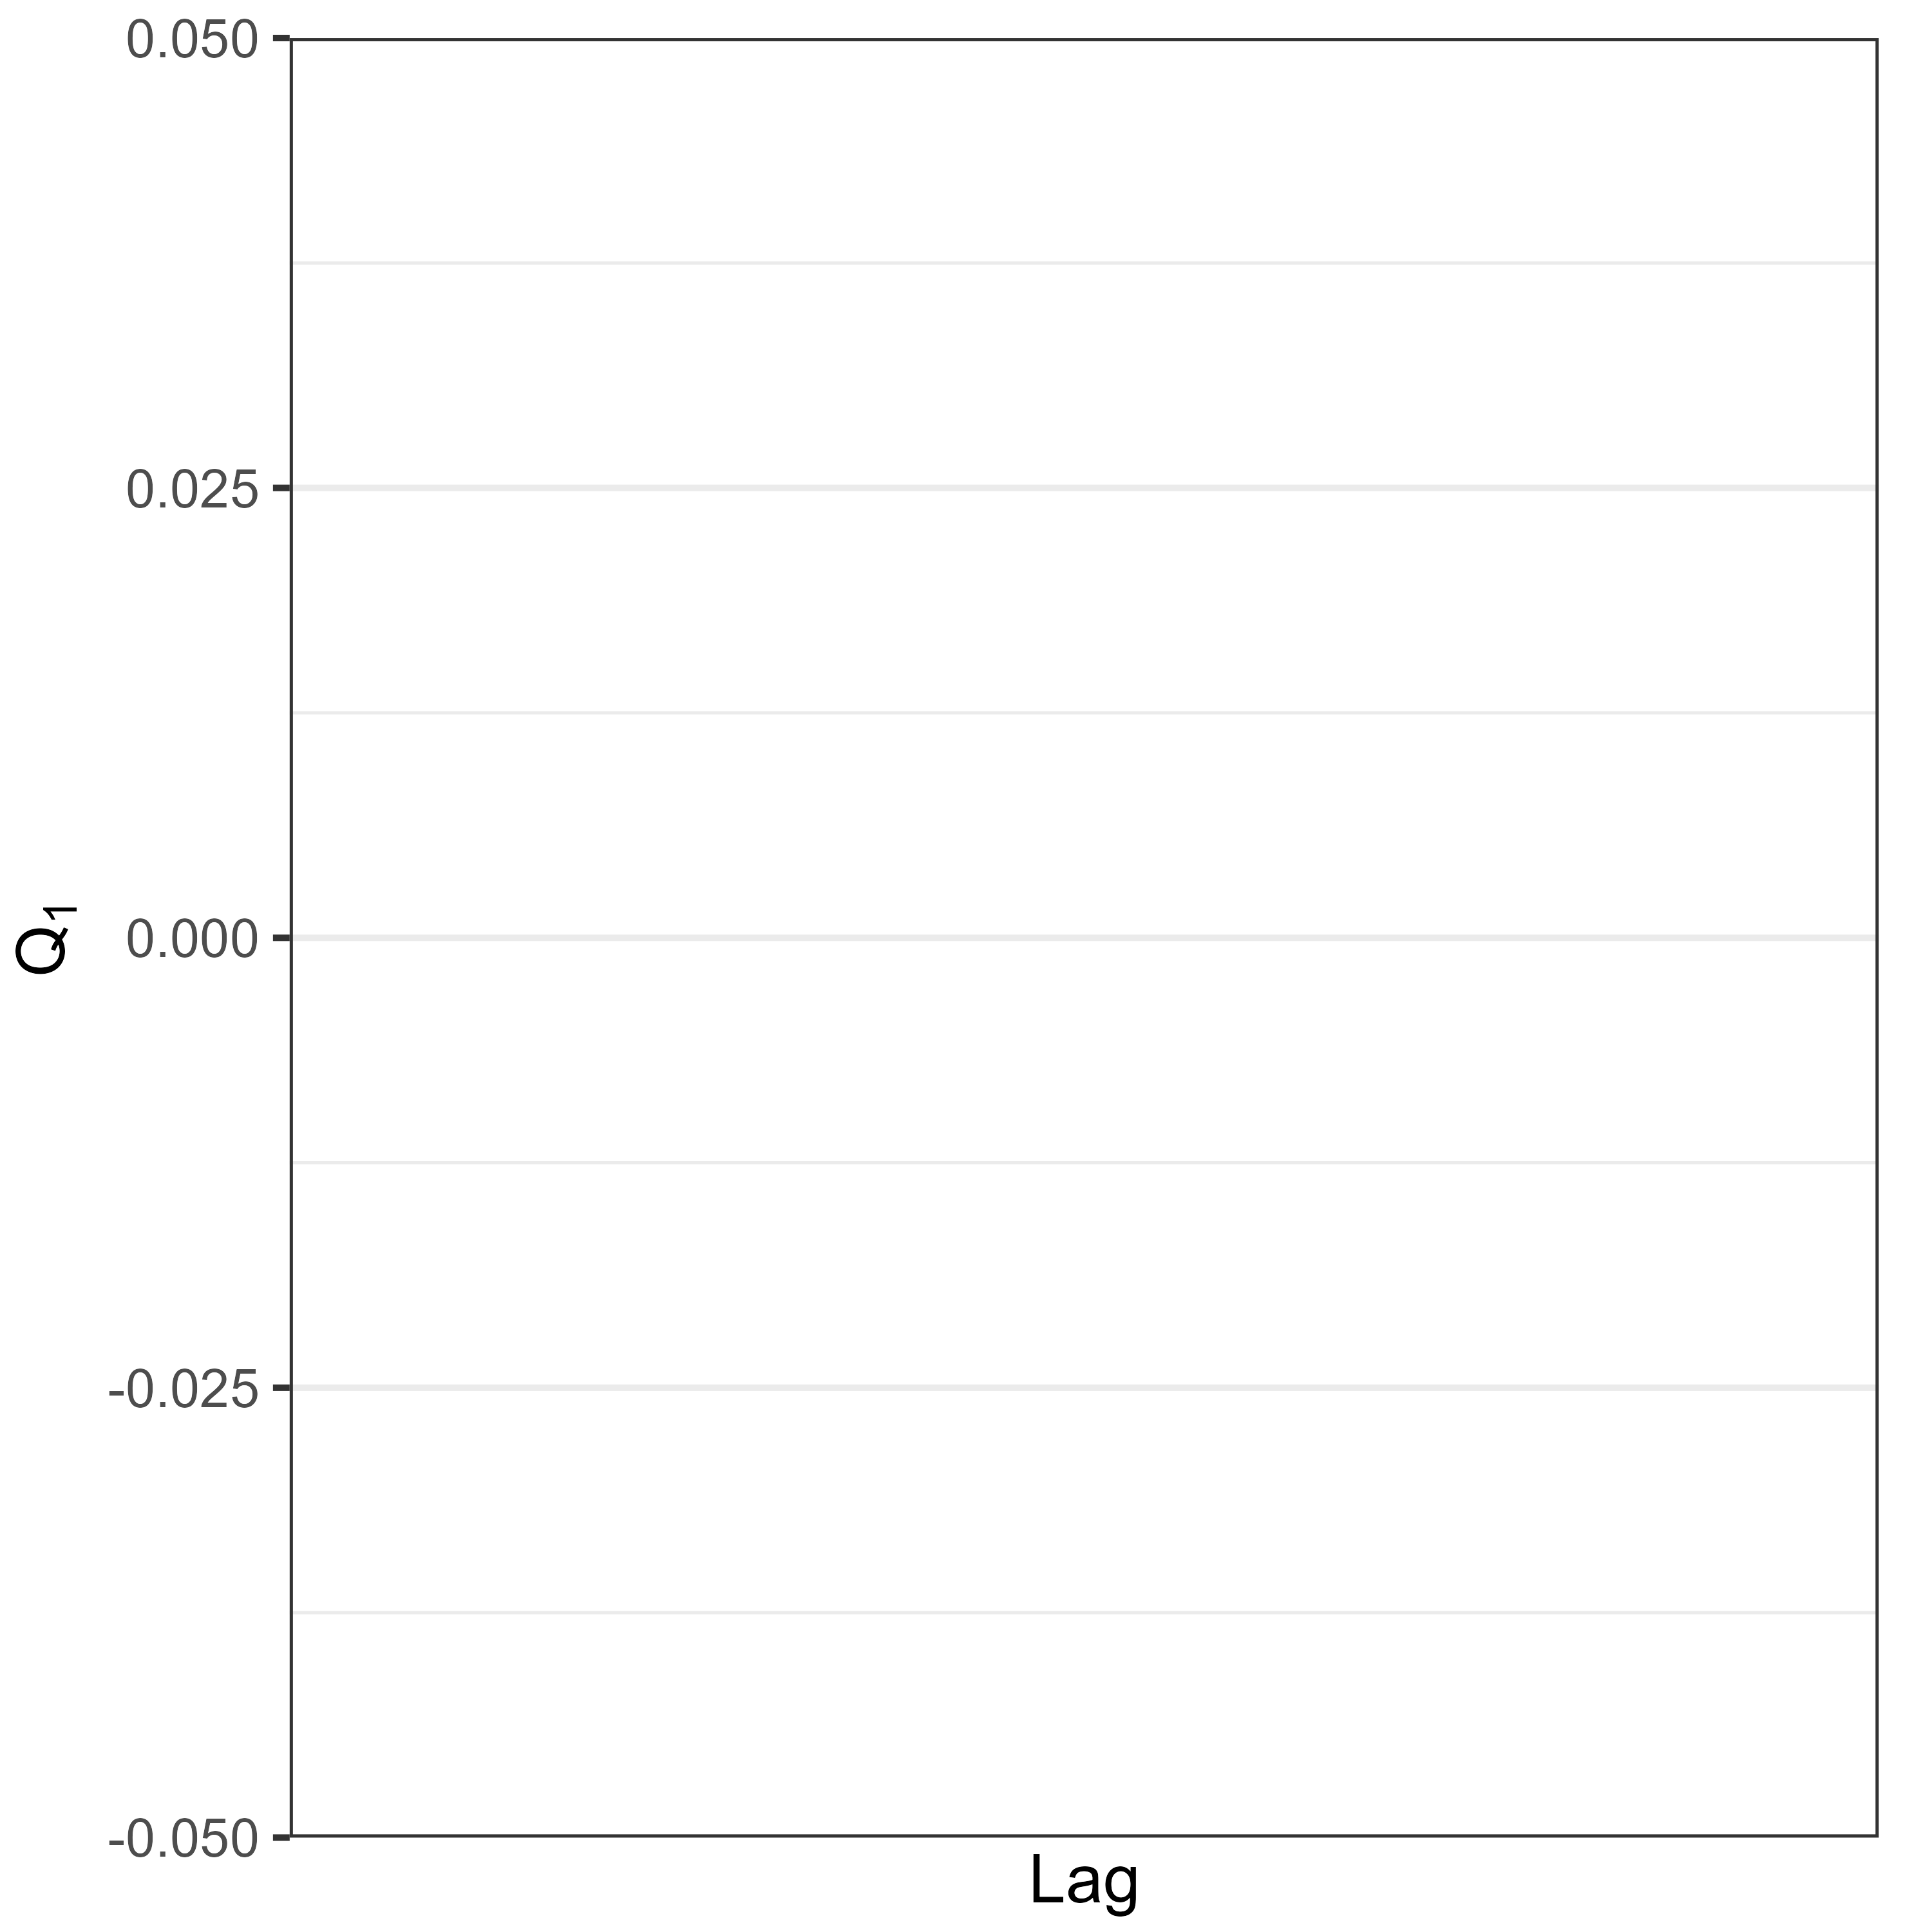
\includegraphics[width=0.45\textwidth]{../figures/acf_Q11.png}
    \caption{Autocorrelation plots for $\lambda$, $A_{11}$, $H_{11}$ and $Q_{11}$.}
\end{figure}

\paragraph{Acceptance rates and effective sample size} The table below summarizes acceptance rates for the Metropolis-Hastings steps (for $\lambda$ and $\mathbf{A}$) and the effective sample size (ESS) for selected components. Values are consistent with good sampler performance.


% Table created by stargazer v.5.2.3 by Marek Hlavac, Social Policy Institute. E-mail: marek.hlavac at gmail.com
% Date and time: Mon, Apr 21, 2025 - 10:38:48 PM
\begin{table}[!htbp] \centering 
  \caption{Acceptance Rates and Effective Sample Size} 
  \label{} 
\begin{tabular}{@{\extracolsep{5pt}} cccc} 
\\[-1.8ex]\hline 
\hline \\[-1.8ex] 
 & Parameter & Acceptance\_Rate & ESS \\ 
\hline \\[-1.8ex] 
1 & A & $0.245$ & $6.426$ \\ 
2 & lambda & $0.940$ & $0.899$ \\ 
\hline \\[-1.8ex] 
\end{tabular} 
\end{table} 
